\begin{figure}[htbp]
\centering
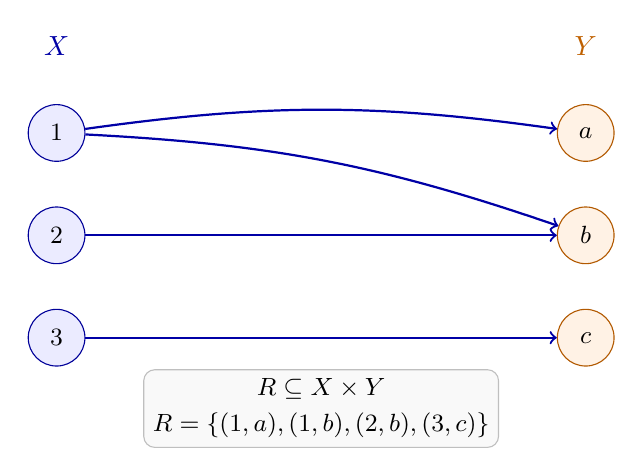
\begin{tikzpicture}[x=1.2cm,y=1cm,font=\small,vertex/.style={circle,draw=blue!60!black,fill=blue!8,minimum size=0.72cm},target/.style={circle,draw=orange!70!black,fill=orange!10,minimum size=0.72cm}]
    \node[font=\bfseries,text=blue!65!black] at (1.6,4.1) {$X$};
    \node[font=\bfseries,text=orange!75!black] at (7.2,4.1) {$Y$};
    \node[vertex] (x1) at (1.6,3) {$1$};
    \node[vertex] (x2) at (1.6,1.7) {$2$};
    \node[vertex] (x3) at (1.6,0.4) {$3$};
    \node[target] (ya) at (7.2,3) {$a$};
    \node[target] (yb) at (7.2,1.7) {$b$};
    \node[target] (yc) at (7.2,0.4) {$c$};
    \draw[->,thick,blue!65!black] (x1) to[bend left=8] (ya);
    \draw[->,thick,blue!65!black] (x1) to[bend left=8] (yb);
    \draw[->,thick,blue!65!black] (x2) -- (yb);
    \draw[->,thick,blue!65!black] (x3) -- (yc);
    \node[draw=gray!50,rounded corners,fill=gray!5,align=center] at (4.4,-0.5) {$R\subseteq X\times Y$\\[2pt]$R=\{(1,a),(1,b),(2,b),(3,c)\}$};
\end{tikzpicture}
\caption{A relation is a selected collection of ordered pairs: each arrow $x\to y$ records one pair $(x,y)\in R$. Unlike a function, a relation may send one source to several targets.}
\label{fig:relation-as-bipartite-graph}
\end{figure}